\chapter{Implementarea platformei Favigon}

\section{Privire de ansamblu asupra implementării}

După etapa de proiectare, implementarea efectivă a platformei a urmărit aceeași idee centrală: fiecare zonă importantă a produsului trebuie să aibă responsabilități clare și puncte de integrare ușor de urmărit. În practică, asta a însemnat că nu a fost dezvoltat întâi un editor izolat și abia apoi restul produsului, ci aplicația a evoluat ca întreg.

Mai exact, partea de autentificare, management de proiecte și persistare a fost dezvoltată relativ devreme, pentru că fără ele editorul ar fi rămas un demo local. Apoi au fost consolidate editorul canvas și suportul pentru export. Într-o etapă ulterioară au fost integrate fluxurile AI și a fost extinsă componenta socială, astfel încât proiectele să poată fi nu doar create, ci și publicate, descoperite și reutilizate.

Rezultatul este o aplicație în care modulele sunt diferite ca rol, dar strâns legate între ele. De exemplu, editorul depinde de proiecte, proiectele depind de autentificare, generarea AI depinde de editor și de modelul intermediar, iar funcțiile sociale depind de modelul relațional al utilizatorilor și proiectelor.

\section{Rutare și pornirea aplicației frontend}

Configurația frontend-ului este definită în \texttt{ApplicationConfig}, prin \texttt{provideRouter}, \texttt{provideHttpClient} cu interceptori și \texttt{provideAnimations}. Alegerea este în linie cu stilul modern Angular bazat pe componente standalone. Din punct de vedere practic, ea reduce nevoia unor module centrale voluminoase și face mai clară relația dintre rutare, infrastructura HTTP și comportamentul global al aplicației.

Un alt detaliu util este activarea \texttt{provideZoneChangeDetection} cu \texttt{eventCoalescing}. Pentru un produs cu editor vizual, optimizarea este relevantă deoarece reduce numărul de actualizări declanșate de evenimente succesive și ajută la păstrarea unei interfețe mai fluide în scenarii de drag, selecție sau input repetat.

Rutarea este organizată astfel încât paginile principale să fie încărcate lazy și protejate diferențiat. Ruta rădăcină nu trimite utilizatorul într-o pagină statică, ci încearcă să încarce utilizatorul curent și redirecționează dinamic fie spre profilul acestuia, fie spre \texttt{/login}. În plus, editorul canvas folosește un \textit{canDeactivate guard} care forțează flush-ul persistenței înainte de părăsirea paginii, ceea ce leagă direct infrastructura de navigare de cerința de robusteză a autosave-ului.

\begin{table}[H]
  \centering
  \caption{Rute frontend principale și rolul lor în aplicație}
  \label{tab:rute-frontend}
  \renewcommand{\arraystretch}{1.15}
  \begin{tabularx}{\textwidth}{>{\RaggedRight\arraybackslash}p{4.2cm}>{\RaggedRight\arraybackslash}p{4.1cm}Y}
    \toprule
    \textbf{Rută} & \textbf{Scop} & \textbf{Observații de acces / navigare} \\
    \midrule
    \path{/login} & autentificare în sistem & \texttt{loginEntryGuard}; evită revenirea inutilă la login \\
    \path{/reset-password} & recuperare acces & rută publică pentru resetarea parolei \\
    \path{/project/:slug} & editorul canvas & \texttt{authGuard} și \texttt{canDeactivate} pentru flush \\
    \path{/project/:slug/preview} & previzualizare HTML & necesită autentificare și randare separată \\
    \path{/explore} & descoperire de proiecte & punct de intrare în zona socială \\
    \path{/settings} & configurări de profil & disponibilă doar utilizatorului autentificat \\
    \path{/stars} & proiecte salvate & afișează bookmark-urile proprii \\
    \path{/:username} & profil public / propriu & destinație implicită după încărcarea sesiunii \\
    \bottomrule
  \end{tabularx}
\end{table}

Interacțiunea dintre rutare și infrastructura HTTP este completată de doi interceptori importanți: unul pentru trimiterea credențialelor către API și altul pentru încercarea automată de refresh atunci când sesiunea curentă expiră. Din punct de vedere al utilizatorului, această logică face ca aplicația să pară mai continuă și mai coerentă; din punct de vedere tehnic, ea mută comportamentele repetitive într-un strat transversal, în loc să fie duplicate în fiecare pagină sau serviciu.

\section{Modulul de autentificare și profil}

\subsection{Fluxurile de bază}

Modulul de autentificare este implementat în jurul `AccountController` și al serviciului `AuthService`. La nivel de API există endpoint-uri pentru register, login, logout, refresh, resetare parolă, setare parolă, schimbare parolă, autentificare prin GitHub și Google, precum și pentru activarea sau dezactivarea autentificării în doi pași.

Pe partea de backend, `AuthService` face mai mult decât o simplă verificare de credențiale. El normalizează datele de intrare, verifică unicitatea utilizatorului, gestionează hash-uirea parolei, tratează fluxurile OAuth, construiește token-urile JWT și emite un token temporar pentru etapa intermediară a autentificării în doi pași. În plus, aceeași zonă gestionează și resetarea parolei prin token transmis prin email.

Din punct de vedere al produsului, autentificarea nu este tratată ca o singură operație de tip ``email + parolă''. În practică, utilizatorii pot intra în sistem prin mai multe căi și pot avea conturi legate la furnizori diferiți. Din acest motiv există și entitatea `LinkedAccount`, folosită pentru asocierea unui utilizator local cu identități externe.

\subsection{JWT în cookie și refresh token}

O decizie importantă a fost transportul token-ului de acces prin cookie HTTP only. În implementare, controller-ul nu întoarce token-ul către frontend pentru stocare manuală în `localStorage`, ci îl plasează în cookie-ul `jwt`. Refresh token-ul este păstrat separat, într-un cookie dedicat cu path limitat la endpoint-ul de refresh.

Această alegere simplifică partea de client și reduce expunerea unor date sensibile în codul din browser. În același timp, introduce și obligația de a trata atent expirațiile și reînnoirea sesiunii. De aceea, în frontend există și interceptorul de refresh, care încearcă revalidarea sesiunii când întâlnește un răspuns care indică expirarea token-ului de acces.

\subsection{Autentificarea în doi pași}

În cadrul proiectului, 2FA este implementat prin cod temporar trimis prin email. La prima vedere, acesta nu este cel mai avansat model posibil, dar pentru scopul aplicației este o soluție rezonabilă și ușor de demonstrat. În plus, implementarea este structurată destul de curat: există flux separat pentru activare, dezactivare și verificare la login, iar token-ul temporar pentru sesiunea de autentificare incompletă este diferit de token-ul normal de acces.

Această funcționalitate nu rămâne la nivel de extensie izolată. Ea este integrată atât în serviciul de autentificare, cât și în controller, în opțiuni și în fluxul de UI, ceea ce îi conferă rolul unei măsuri reale de securitate operațională.

\subsection{Profilul utilizatorului}

Pe lângă autentificare, utilizatorul își poate administra profilul: nume afișat, bio, imagine și legături OAuth. `UsersController` expune endpoint-uri pentru profilul curent, încărcarea imaginii de profil, căutarea de utilizatori și vizualizarea profilurilor publice. În plus, există endpoint-uri pentru follow și unfollow, precum și pentru listele de followers și following.

Această parte a aplicației are un rol dublu. Pe de o parte este o funcționalitate de produs normală. Pe de altă parte, ea oferă baza pentru zona socială și pentru ideea că proiectele au autori, pot fi urmărite și pot circula între utilizatori.

\section{Gestionarea proiectelor}

\subsection{Ciclul de viață al proiectelor}

`ProjectService` este una dintre cele mai importante piese din backend, deoarece concentrează logica legată de proiecte. El gestionează crearea proiectului, actualizarea metadatelor, ștergerea, salvarea designului, salvarea thumbnail-ului, upload-ul de imagini, bookmark-urile, like-urile și operația de fork.

La creare, proiectul primește un slug unic derivat din nume. La modificare, dacă numele se schimbă, slug-ul este recalculat. La ștergere, serviciul se ocupă și de curățarea asset-urilor asociate. Acest detaliu este important deoarece evită acumularea de fișiere orfane și arată că proiectul nu tratează persistența doar la nivel de bază de date, ci și la nivelul fișierelor încărcate.

\subsection{Persistarea designului}

Pentru design-ul propriu-zis al unui proiect, backend-ul păstrează JSON-ul serializat în câmpul `DesignJson` al entității `Project`. Pe frontend, `CanvasPersistenceService` coordonează încărcarea, transformarea și salvarea acestui document.

Un aspect important este că salvarea nu este exclusiv manuală. Editorul folosește persistare automată cu debounce și mecanisme de flush atunci când utilizatorul părăsește pagina sau proiectul trebuie sincronizat imediat. Acest comportament este important pentru UX. Dacă utilizatorul lucrează într-un editor de design și trebuie să apese explicit \textit{Save} după fiecare pas important, experiența devine artificială și fragilă.

În implementare, persistarea automată este tratată explicit prin parametri observabili în cod: schimbările relevante programează o salvare după 500 ms, flush-ul așteaptă cel mult 4 s finalizarea persistenței, iar la erori temporare se folosesc până la 4 reîncercări cu backoff exponențial pornind de la 2 s. Serviciul gestionează separat stările de \textit{isSaving}, persistarea la ieșirea din pagină și generarea de thumbnail-uri după perioade scurte de inactivitate. Aceste detalii transformă editorul dintr-un demo interactiv într-un subsistem care poate susține utilizare repetată.

\subsection{Thumbnail și asset-uri}

Fiecare proiect poate avea și thumbnail. În editor, thumbnail-ul este generat automat pornind din canvas, inclusiv printr-o variantă bazată pe `html2canvas`. Pe backend, fișierul este salvat separat, iar la update se invalidează vechiul `ThumbnailDataUrl` dacă este cazul.

În plus, proiectul suportă upload de imagini pentru asset-uri folosite în design. Validarea fișierelor se face în backend, iar stocarea este abstractizată printr-un serviciu dedicat. Această decizie a fost utilă pentru că a evitat legarea prea strânsă a logicii de proiecte de detaliile concrete ale fișierelor.

Un detaliu important, mai puțin vizibil în interfață, este ciclul de viață al asset-urilor. La resalvarea designului, backend-ul compară asset-urile prezente în documentul nou cu cele din versiunea anterioară și poate elimina resursele care au devenit orfane. În mod similar, la ștergerea unui proiect sau a unui cont, sunt curățate atât asset-urile proiectelor, cât și imaginea de profil a utilizatorului. Această zonă nu schimbă experiența vizuală în mod direct, dar este importantă pentru a arăta că aplicația tratează responsabil și consistența stocării de fișiere.

\section{Funcționalități sociale și explorare}

Componenta socială este construită peste fluxurile de explorare, proiecte și utilizatori, împreună cu serviciile și repository-urile aferente. În această zonă, utilizatorii pot vedea proiecte populare sau recomandate, pot descoperi alți utilizatori, pot aprecia proiecte, le pot salva și le pot reutiliza prin fork.

Deși această zonă nu este nucleul tehnic al lucrării, ea schimbă semnificativ caracterul produsului. Fără ea, Favigon ar fi rămas un editor personal. Cu ea, proiectul capătă logică de comunitate: există autori, conținut public, indicatori de interes și relații între utilizatori.

În implementare, `ExploreService` tratează separat trei fluxuri: proiecte \textit{trending}, proiecte recomandate și utilizatori sugerați. Pentru proiectele populare este folosit un set limitat de rezultate, potrivit pentru afișarea rapidă a conținutului public. Pentru recomandări, backend-ul verifică mai întâi dacă utilizatorul autentificat urmărește deja alte conturi; dacă da, încearcă să construiască un răspuns personalizat, iar dacă nu există bază suficientă sau utilizatorul este anonim, revine la o selecție generală de proiecte recente și relevante. Pentru sugestiile de persoane, serviciul returnează informații derivate precum numărul de urmăritori, numărul de proiecte publice și starea \textit{isFollowedByCurrentUser}. Această logică oferă zonei `explore` un comportament mai apropiat de un produs real decât de o simplă listă statică.

Operația de fork este deosebit de interesantă deoarece leagă partea socială de partea de producție. Când un utilizator face fork la un proiect public, sistemul creează un nou proiect privat pentru el, cu design-ul copiat și cu legătura către proiectul-sursă. Astfel, reutilizarea nu este doar conceptuală, ci concretă și trasabilă.

\begin{figure}[H]
  \centering
  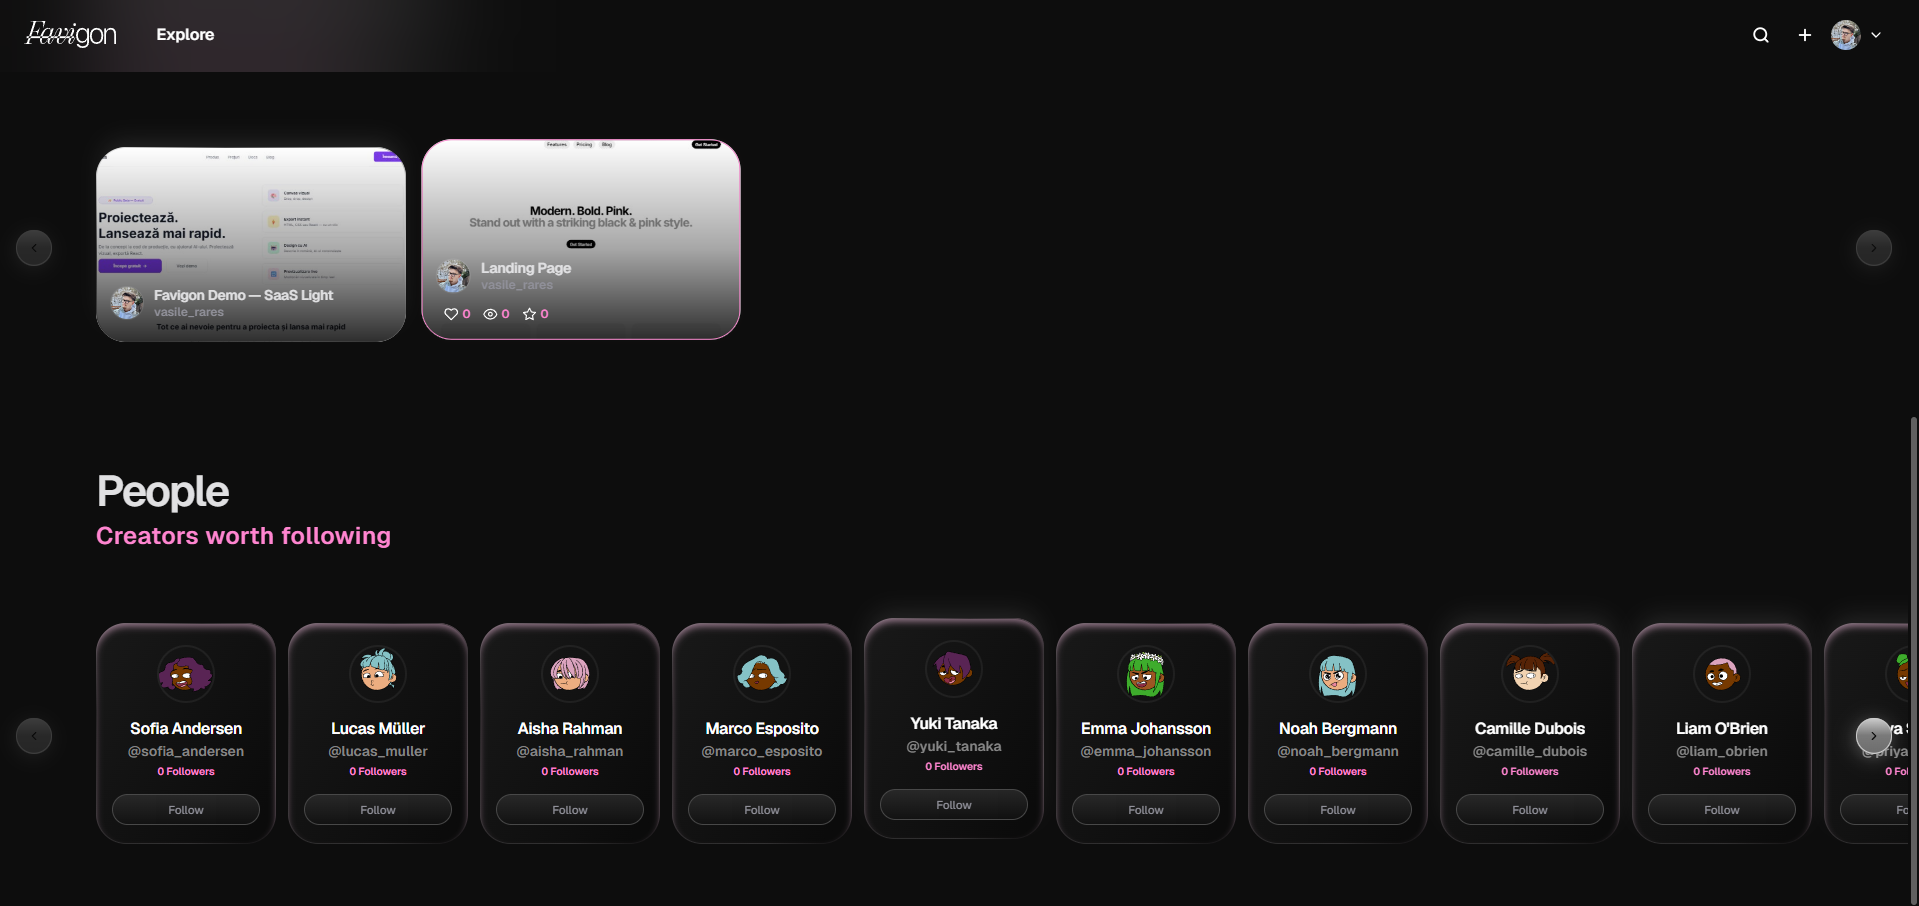
\includegraphics[width=0.96\textwidth]{images/explore_page.png}
  \caption{Interfața paginii Explore, cu proiecte publice și utilizatori sugerați}
  \label{fig:explore-page}
\end{figure}

\section{Suprafața API și distribuția responsabilităților}

Din perspectiva backend-ului, aplicația expune o suprafață REST suficient de largă încât să merite descrisă separat. În forma actuală, API-ul este împărțit în șase controllere principale. Unele acoperă autentificarea și profilul, altele gestionează proiectele și componenta socială, iar cele rămase tratează generarea asistată de AI și exportul în cod.

Distribuția responsabilităților pe controllere are un rol important în claritatea implementării. Zonele costisitoare sau sensibile, precum AI-ul și convertorul, sunt separate de ciclul de viață al proiectelor. În același timp, controllerele de produs, cum sunt cele pentru proiecte și utilizatori, pot rămâne focalizate pe resursele pe care le gestionează. Astfel, API-ul nu devine o colecție arbitrară de endpoint-uri, ci o hartă destul de coerentă a capabilităților aplicației.

\begin{table}[H]
  \centering
  \caption{Controllere API și responsabilitățile lor dominante}
  \label{tab:controllere-api}
  \renewcommand{\arraystretch}{1.15}
  \begin{tabularx}{\textwidth}{>{\RaggedRight\arraybackslash}p{2.9cm}>{\RaggedRight\arraybackslash}p{5.1cm}Y}
    \toprule
    \textbf{Controller} & \textbf{Resurse / operații principale} & \textbf{Observații utile} \\
    \midrule
    Account & autentificare, sesiune, parole, OAuth, 2FA & concentrează logica de intrare în sistem \\
    Projects & CRUD proiecte, design, asset-uri, reacții, fork & controllerul cel mai bogat din zona de produs \\
    Users & profil curent/public, follow, linked accounts & leagă identitatea utilizatorului de zona socială \\
    Explore & trending, recomandări și sugestii de utilizatori & pune în valoare date agregate și filtrate, nu doar resurse brute \\
    AI design & generare directă, streaming, pipeline pe faze & include atât răspuns sincron, cât și SSE incremental \\
    Converter & validare IR, export HTML/React/Angular, multi-page & separă clar validarea de generarea finală \\
    \bottomrule
  \end{tabularx}
\end{table}

În implementare se observă și diferențierea infrastructurală a acestor zone. Controllerul AI este protejat atât prin autorizare, cât și prin politica dedicată de rate limiting \texttt{ai}. Controllerul de conversie are propria politică \texttt{converter}, iar \texttt{ProjectsController} aplică și limite diferite de dimensiune pentru upload de imagini, salvare design, flush și thumbnail. Aceste detalii arată că separarea controllerelor nu este doar conceptuală, ci are și efecte practice asupra securității, costului și fiabilității API-ului.

Dacă diagrama de arhitectură din capitolul precedent arată straturile mari, Figura~\ref{fig:backend-structural} coboară un nivel și sintetizează colaborarea dintre clasele și serviciile dominante din fluxurile AI și export. Nu este o diagramă exhaustivă a întregului backend, ci o vedere structurală orientată pe subsistemele cele mai relevante pentru contribuția tehnică a lucrării.

\begin{figure}[H]
  \centering
  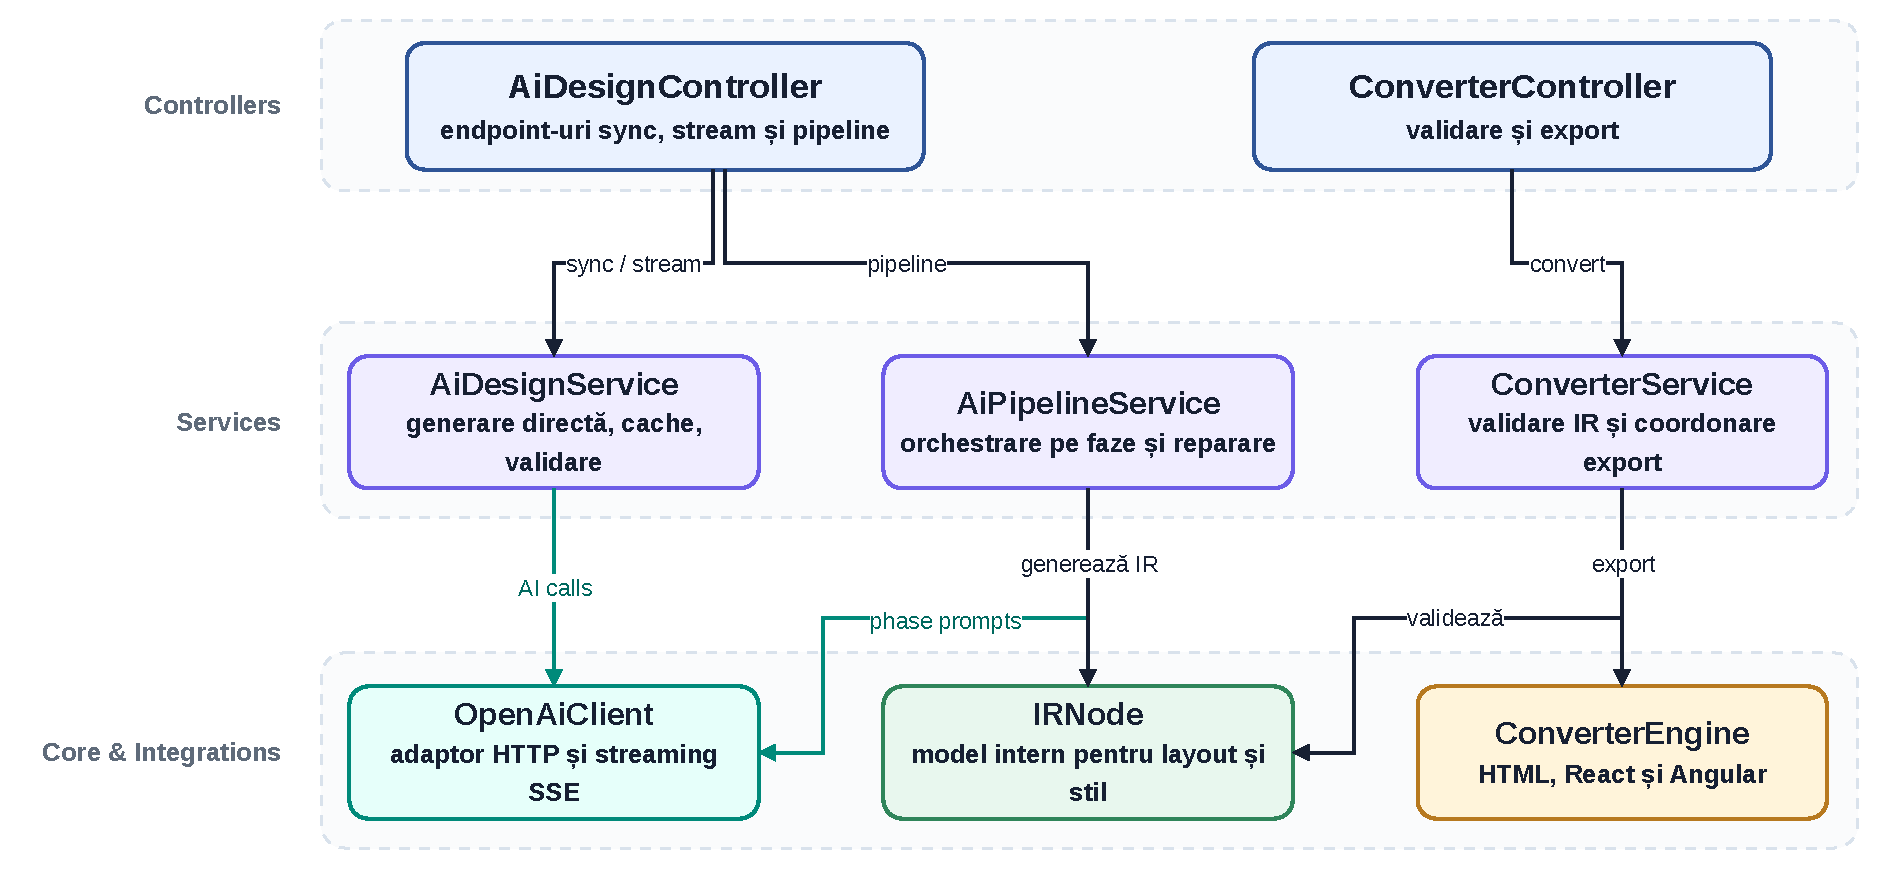
\includegraphics[width=0.96\textwidth]{diagrams/backend-structural.drawio.pdf}
  \caption{Vedere structurală simplificată a principalelor clase și servicii backend}
  \label{fig:backend-structural}
\end{figure}

\section{Editorul canvas}

\subsection{Rolul editorului în întregul produs}

Editorul canvas este zona cea mai complexă din frontend și, în mod realist, centrul aplicației. În jurul lui gravitează generarea AI, persistarea, exportul și o mare parte din interacțiunile vizuale ale utilizatorului. În implementare, pagina principală a editorului (`CanvasPage`) este o componentă mare, dar ea funcționează mai mult ca punct de orchestrare decât ca loc în care se află toată logica.

Practic, componenta injectează o suită întreagă de servicii: stare editor, viewport, istoric, clipboard, gesturi, context menu, persistare, generare, manager de pagini, stilizare DOM și altele. Separarea urmărește principiile interacțiunii de tip \textit{direct manipulation}, unde utilizatorul operează pe obiecte vizibile, primește feedback imediat și poate reveni rapid asupra acțiunilor \cite{shneiderman1983direct}. În același timp, păstrarea unui model intern separat de suprafața vizuală apropie editorul de direcțiile discutate în literatura despre combinarea editării directe cu reprezentări programabile \cite{chugh2016programmatic}. Principalele servicii implicate sunt sintetizate în Figura~\ref{fig:canvas-servicii}.

\begin{figure}[H]
  \centering
  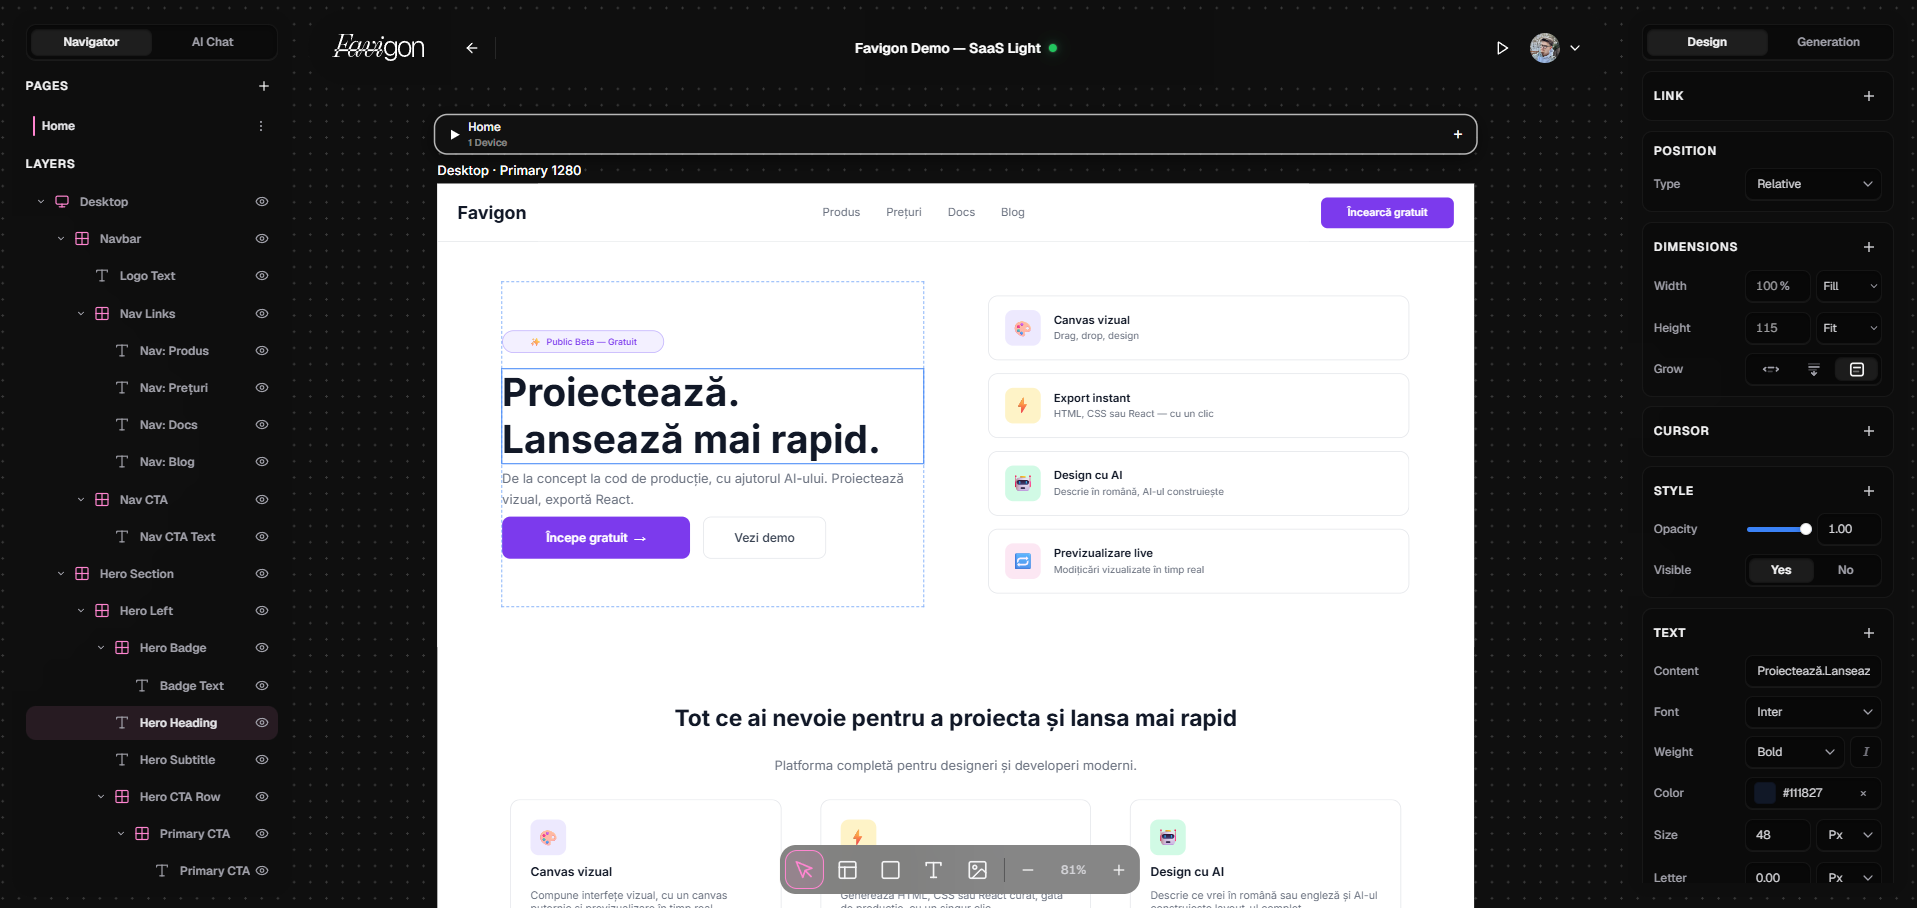
\includegraphics[width=0.96\textwidth]{images/canvas_editor.png}
  \caption{Interfața editorului canvas în timpul editării unui proiect}
  \label{fig:canvas-editor}
\end{figure}

\subsection{Starea editorului}

`CanvasEditorStateService` păstrează semnalele principale ale editorului: paginile, pagina curentă, elementele selectate, unealta curentă și alte stări derivate. Faptul că starea este separată într-un serviciu dedicat face posibilă partajarea ei între mai multe comportamente fără a transmite manual date prin multe nivele de componente.

Pe lângă starea explicită, editorul folosește și multe valori derivate: elementul curent, limitele selecției, lista de elemente vizibile, hărți auxiliare pentru copii, indexări rapide și stări temporare de drag sau resize. În cod se vede clar că aceste structuri sunt tratate ca parte din modelul intern al editorului, nu ca simple variabile locale.

\subsection{Viewport, selecție și gesturi}

Pentru ca editorul să fie util, utilizatorul trebuie să poată naviga în canvas, să selecteze elemente și să le manipuleze natural. `CanvasViewportService` controlează zoom-ul, offset-ul și proprietățile CSS asociate. `CanvasGestureService` gestionează drag, resize, rotate, editarea de text și calculul limitelor pentru overlay-uri.

O problemă practică interesantă a fost sincronizarea dintre modelul intern și limitele reale din DOM, mai ales pentru elemente transformate sau pentru copii din layout-uri flexibile. De aceea, în implementare există noțiuni precum \textit{stable selection bounds}, cache pentru limite și mecanisme speciale pentru cazurile în care măsurarea live ar produce efecte vizuale nedorite. Este un exemplu de complexitate care nu apare în descrierea de nivel înalt, dar devine foarte concretă într-un editor bazat pe gesturi, selecție și feedback imediat.

\subsection{Istoric și clipboard}

`CanvasHistoryService` și `CanvasClipboardService` susțin operații de tip undo, redo, copy și paste. Din punct de vedere al utilizatorului, acestea sunt funcții de bază. Din punct de vedere intern, ele sunt importante pentru că obligă sistemul să poată captura și reaplica stări coerente ale documentului.

Pentru istoric, soluția folosită este bazată pe snapshot-uri ale stării relevante. Nu este cea mai sofisticată variantă posibilă, dar pentru proiectul de față oferă un raport bun între simplitate și control. În plus, istoricul este suficient de clar încât să poată fi restaurat și după reîncărcarea proiectului.

\subsection{Managementul paginilor}

Editorul nu se limitează la o singură pagină. `CanvasPageManagerService` și serviciile asociate permit existența mai multor pagini în același proiect, schimbarea paginii active și organizarea elementelor pe pagini. Această decizie influențează și exportul, deoarece face posibilă generarea multi-page în backend.

Din perspectiva lucrării, suportul multi-page este important deoarece mută Favigon din zona unui simplu constructor de ecrane izolate spre zona unui sistem care poate descrie un mic site sau o mică aplicație cu mai multe puncte de intrare.

\subsection{Preview-ul interactiv}

Pe lângă editorul propriu-zis, aplicația include și o pagină de preview separată (`CanvasPreviewPage`), folosită atât de autorul proiectului, cât și de vizitatorii care accesează un proiect public. În loc să redea direct structura internă a canvas-ului, această pagină reconstruiește reprezentarea intermediară pentru pagina selectată și cere backend-ului generarea HTML/CSS. Rezultatul este injectat într-un `iframe` prin `srcdoc`, ceea ce permite observarea produsului într-un mediu mai apropiat de randarea finală decât suprafața de editare.

Preview-ul nu este doar o captură statică. El permite schimbarea paginii curente, selectarea unui cadru de vizualizare, redimensionarea viewport-ului și navigarea între pagini prin link-uri interne, interceptate prin `postMessage` între `iframe` și aplicație. În plus, pentru proiectele publice, aceeași pagină expune acțiuni de tip like, star și fork. Din acest motiv, preview-ul funcționează și ca punte între editor, conversie și partea socială a produsului.

\begin{figure}[H]
  \centering
  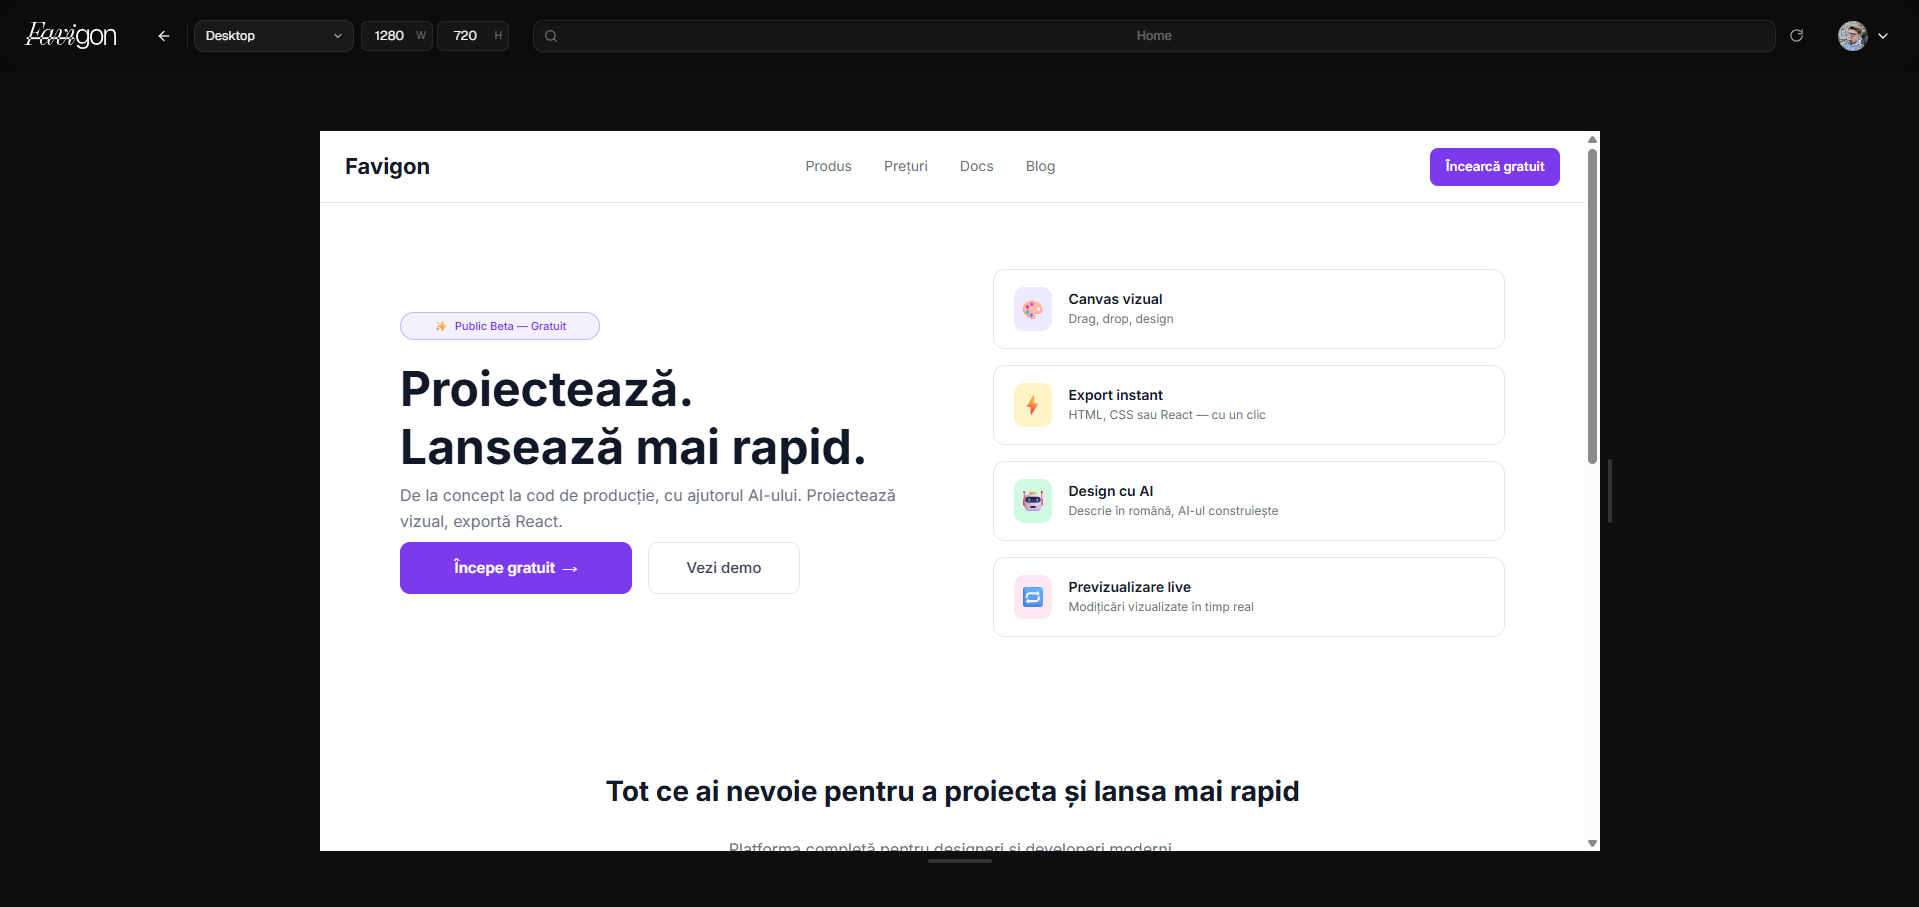
\includegraphics[width=0.96\textwidth]{images/project_preview.png}
  \caption{Pagina de preview folosită pentru vizualizarea rezultatului generat}
  \label{fig:project-preview}
\end{figure}

\subsection{Persistare și integrare cu restul aplicației}

Editorul nu este un spațiu închis. El comunică permanent cu serviciile de proiect, cu zona de preview și cu motorul de conversie. `CanvasPersistenceService` este legătura principală dintre starea editorului și backend. `CanvasGenerationService` este puntea spre export. `CanvasAiChatPersistenceService` și istoricul extind editorul dincolo de o simplă editare de suprafață.

Din punct de vedere practic, această integrare a fost mai grea decât scrierea unui editor minimal. Nu era suficientă mutarea unui element pe ecran; era necesară și posibilitatea de salvare, validare, export și reîncărcare a rezultatului fără inconsistențe majore.

\subsection{Persistența locală a conversației AI}

O extensie utilă a editorului este păstrarea locală a conversației AI și a contextului asociat. `CanvasAiChatPersistenceService` folosește `IndexedDB` pentru a salva, per proiect, mesajele recente, promptul aflat în lucru, modelul selectat și tab-ul activ al interfeței. Persistarea este făcută cu debounce de 300 ms, iar la restaurare sunt acceptate doar intrările mai noi de 7 zile. În plus, serviciul limitează mesajele păstrate la 40 și normalizează lungimea textelor, pentru a evita acumularea necontrolată de date în browser.

Această decizie completează bine autosave-ul clasic al designului. Documentul proiectului rămâne în backend, pentru a putea fi sincronizat și exportat, în timp ce conversația AI și contextul ei imediat rămân locale, ceea ce reduce trafic inutil și permite reluarea rapidă a sesiunii după reîncărcarea editorului. Împreună cu restaurarea istoricului și cu flush-ul la ieșire din pagină, rezultă un comportament mult mai apropiat de un instrument de lucru continuu decât de un simplu demo de generare.

\begin{figure}[H]
  \centering
  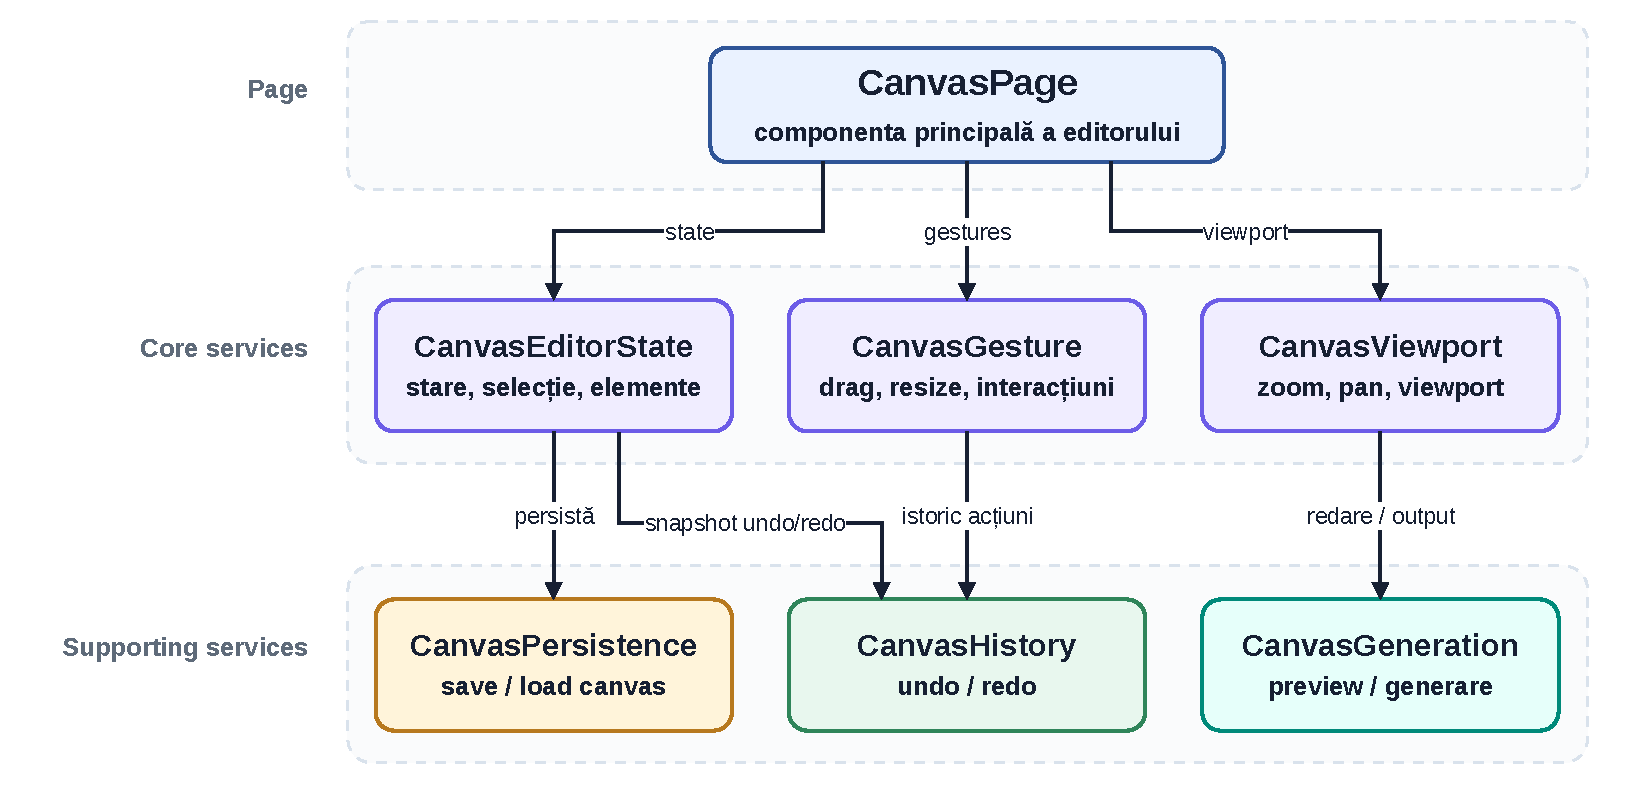
\includegraphics[width=0.96\textwidth]{diagrams/canvas-servicii.drawio.pdf}
  \caption{Servicii principale implicate în funcționarea editorului canvas}
  \label{fig:canvas-servicii}
\end{figure}

\section{Decizii de implementare cu impact major}

Privind la implementarea efectivă, există câteva decizii care au avut impact direct asupra stabilității și clarității codului.

Prima este faptul că logica specifică canvas-ului a fost păstrată în interiorul feature-ului `canvas`. În multe proiecte, utilitarele și serviciile migrează rapid spre zone generice, dar aici asta ar fi redus claritatea.

A doua este persistarea automată cu retry și flush controlat. Nu este o funcție spectaculoasă în demo, dar este foarte importantă în utilizare reală.

A treia este tratarea editorului ca pe o sumă de servicii coordonate, nu ca pe o singură componentă imensă care face totul. Deși `CanvasPage` rămâne o componentă mare, mare parte din comportament este împinsă în servicii.

A patra este integrarea atentă dintre proiecte, thumbnail-uri și asset-uri. Fără această zonă, editorul ar fi avut o viață scurtă în afara unei sesiuni locale.

\section{Concluzii intermediare}

Implementarea platformei arată că Favigon este mai mult decât un proof of concept pentru generare AI. Autentificarea, proiectele, profilurile, funcțiile sociale și editorul canvas formează împreună baza produsului. În această bază, editorul este modulul cel mai complex, dar el nu ar avea aceeași valoare fără restul infrastructurii de produs.

Capitolul următor tratează componenta care diferențiază cel mai mult proiectul din punct de vedere tehnic: generarea asistată de AI și conversia interfețelor în cod.
